\documentclass[border=4pt,12pt]{standalone}
% House style for redrawn exam diagrams (diagram-v4: 0.4pt lines, filled -latex arrows, fine dashes; stipple and hatching drawn as real dots/lines (no PDF/SVG patterns, so they render in every browser and at any scale); transparent background). Every figure \input's this.
\usepackage{amsmath,amssymb}
\usepackage{txfonts}
\usepackage{pdfrender,xcolor}
% \halo{text}: label on shading. The shading stops just around each letter's outline (a thin knock-out that follows the
% glyphs, like the papers' typesetting), never a box. Owner: "I don't want a box around the text".
\newcommand{\halo}[1]{\leavevmode\rlap{\pdfrender{TextRenderingMode=2,LineWidth=2.2pt,LineJoinStyle=1,StrokeColor=white,FillColor=white}#1}#1}
\usepackage{tikz,pgfplots}
\pgfplotsset{compat=1.18}
\usetikzlibrary{arrows.meta,calc,angles,quotes,patterns,patterns.meta,intersections,positioning,decorations.markings,shapes.geometric}
% Stipple and hatching are drawn as actual dots / lines clipped to the region (path picture), NOT as pattern fills:
% SVG <pattern> fills vanish or blur when browsers scale the image, so the owner could not see the shading.
% Each dot is a 0.72pt square (keeps SVGs small; reads as a dot at print size). Dots sit on one global staggered grid, so neighbouring regions line up.
\makeatletter
\newdimen\ex@x \newdimen\ex@y \newdimen\ex@xa \newdimen\ex@ya \newdimen\ex@xb \newdimen\ex@yb \newcount\ex@row
\def\exam@stipplecolor{black!75}\def\exam@dotr{0.42pt}\def\exam@dotgap{2.5}
\def\ex@rowdots{\ifdim\ex@x<\ex@xb \pgfpathrectangle{\pgfqpoint{\dimexpr\ex@x-0.36pt\relax}{\dimexpr\ex@y-0.36pt\relax}}{\pgfqpoint{0.72pt}{0.72pt}}\advance\ex@x by \exam@dotgap pt\relax\expandafter\ex@rowdots\fi}
\def\exam@stipple{%
  \pgftransformreset% dots are sized in real points even inside scaled pictures
  \pgfpointanchor{path picture bounding box}{south west}\ex@xa=\pgf@x \ex@ya=\pgf@y
  \pgfpointanchor{path picture bounding box}{north east}\ex@xb=\pgf@x \ex@yb=\pgf@y
  \pgfsetfillcolor{\exam@stipplecolor}\pgfmathsetmacro\ex@h{\exam@dotgap/2}%
  \pgfmathtruncatemacro\ex@r{floor(\ex@ya/\ex@h)-1}\ex@row=\ex@r\relax
  \ex@y=\ex@r\dimexpr\ex@h pt\relax
  \loop\ifdim\ex@y<\ex@yb
    \pgfmathtruncatemacro\ex@c{floor(\ex@xa/\exam@dotgap)-1}\ex@x=\ex@c\dimexpr\exam@dotgap pt\relax
    \ifodd\ex@row \advance\ex@x by \ex@h pt\fi
    \ex@rowdots
    \advance\ex@y by \ex@h pt \advance\ex@row by 1
    \ifnum\numexpr\ex@row-(\ex@row/4)*4\relax=0 \pgfusepath{fill}\fi% flush every 4 rows: bounded TeX memory, few clip copies in the SVG
  \repeat\pgfusepath{fill}}
\newdimen\ex@d
\def\exam@hatch#1{% #1 = 1 for /, -1 for \ ; lines 45 degrees, 3pt apart
  \pgftransformreset
  \pgfpointanchor{path picture bounding box}{south west}\ex@xa=\pgf@x \ex@ya=\pgf@y
  \pgfpointanchor{path picture bounding box}{north east}\ex@xb=\pgf@x \ex@yb=\pgf@y
  \ex@d=\dimexpr\ex@yb-\ex@ya\relax \ex@x=\dimexpr\ex@xa-\ex@d\relax
  \loop\ifdim\ex@x<\ex@xb
    \ifnum#1>0 \pgfpathmoveto{\pgfqpoint{\ex@x}{\ex@ya}}\pgfpathlineto{\pgfqpoint{\dimexpr\ex@x+\ex@d\relax}{\ex@yb}}%
    \else \pgfpathmoveto{\pgfqpoint{\ex@x}{\ex@yb}}\pgfpathlineto{\pgfqpoint{\dimexpr\ex@x+\ex@d\relax}{\ex@ya}}\fi
    \advance\ex@x by 4.24pt
  \repeat
  \pgfsetlinewidth{0.4pt}\pgfsetstrokecolor{black}\pgfusepath{stroke}}
\def\examstipple{\exam@stipple}\def\examhatch{\exam@hatch}\def\examsetstipplecolor#1{\def\exam@stipplecolor{#1}}\def\examsetdotgap#1{\def\exam@dotgap{#1}}
\makeatother
% (legacy pattern kept for old files)
% staggered stipple like the NESA papers' dotted shading
\pgfdeclarepatternformonly{exam stipple}{\pgfpointorigin}{\pgfqpoint{2.2pt}{2.2pt}}{\pgfqpoint{2.2pt}{2.2pt}}{%
  \pgfpathcircle{\pgfqpoint{0.55pt}{0.55pt}}{0.42pt}\pgfpathcircle{\pgfqpoint{1.65pt}{1.65pt}}{0.42pt}\pgfusepath{fill}}
\tikzset{
  every picture/.style={line width=0.6pt, >={Latex[length=2mm,width=1.3mm]}},
  curve/.style={line width=0.6pt},
  open arrow/.style={-{Latex[length=2mm,width=1.3mm]}},  % owner: filled -latex heads everywhere, no open chevrons
  aux/.style={dash pattern=on 2pt off 1.5pt, line width=0.6pt},
  shade/.code={\def\exA{#1}\def\exB{none}\ifx\exA\exB\else\pgfkeysalso{fill=black!18}\fi},
  shade/.default=on,
  shade dots/.style={fill=none, path picture={\examstipple}},
  stipple color/.code={\examsetstipplecolor{#1}},
  stipple gap/.code={\examsetdotgap{#1}},
  shade dense dots/.style={fill=none, stipple gap=1.6, path picture={\examstipple}},
  shade hatch/.style={fill=none, path picture={\examhatch{1}}},
  shade hatch reverse/.style={fill=none, path picture={\examhatch{-1}}},
  shade solid/.style={fill=black},
  pt/.style={circle, fill, inner sep=1.1pt},
  open pt/.style={circle, draw, fill=white, inner sep=1.1pt},
}
\pgfplotsset{
  exam axes/.style={axis lines=middle, axis line style={->}, xlabel={$x$}, ylabel={$y$},
    xlabel style={anchor=west}, ylabel style={anchor=south}, tick label style={font=\small},
    every axis plot/.append style={line width=0.6pt, black}, samples=200, clip=false,
    enlargelimits=false, axis on top},
}

\begin{document}
% crop pixels, y down: X(x)=250.5+78.75x, Y(y)=371.5-78.75y; curve traced from the crop and spline-smoothed
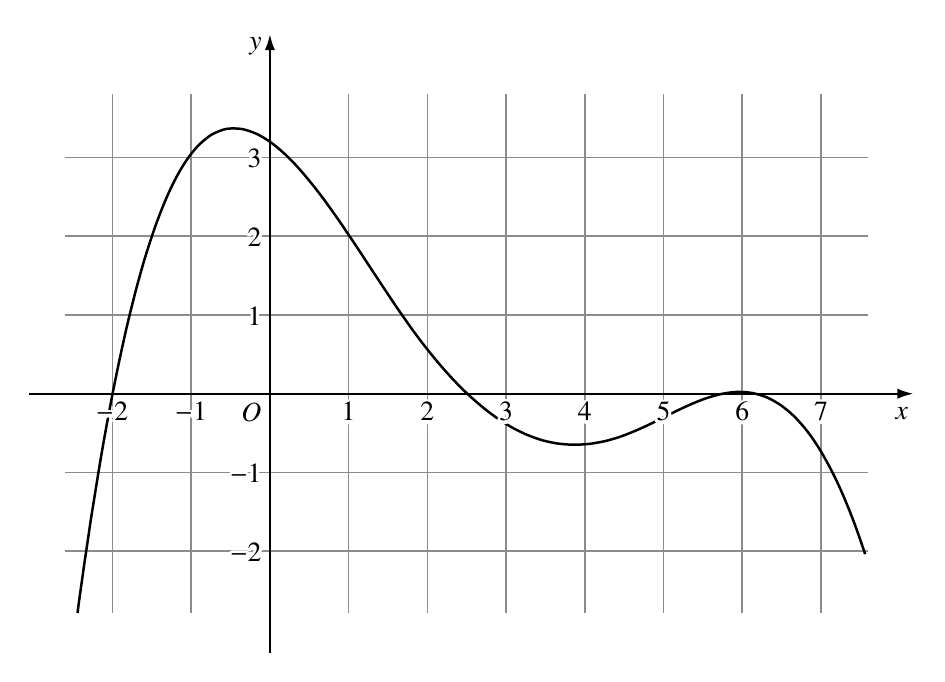
\begin{tikzpicture}[x=0.0127cm, y=-0.0127cm]
  \foreach \i in {-2,-1,1,2,...,7} \draw[black!45] ({250.5+78.75*\i},72) -- ({250.5+78.75*\i},591);
  \foreach \j in {-2,-1,1,2,3} \draw[black!45] (46,{371.5-78.75*\j}) -- (849,{371.5-78.75*\j});
  \draw[->] (9,371.5) -- (894,371.5);
  \draw[->] (250.5,631) -- (250.5,12);
  \draw[line width=0.9pt] plot[smooth] coordinates {(58.0,590.9) (60.1,575.2) (62.3,559.6) (64.5,544.0) (66.8,528.4) (69.1,512.8) (71.4,497.2) (73.9,481.6) (76.4,466.1) (78.9,450.5) (81.5,435.0) (84.2,419.4) (87.0,403.9) (89.9,388.4) (92.8,372.9) (95.9,357.5) (99.1,342.0) (102.4,326.6) (105.8,311.2) (109.4,295.8) (113.2,280.5) (117.1,265.3) (121.3,250.1) (125.7,234.9) (130.5,219.9) (135.5,205.0) (141.0,190.2) (147.0,175.6) (153.6,161.3) (161.1,147.4) (169.7,134.2) (179.9,122.2) (192.2,112.3) (206.8,106.6) (222.4,106.7) (237.3,111.6) (250.9,119.7) (263.1,129.6) (274.4,140.6) (284.9,152.4) (294.9,164.6) (304.5,177.1) (313.7,189.9) (322.7,202.8) (331.5,215.9) (340.3,229.0) (348.9,242.2) (357.6,255.4) (366.3,268.5) (375.0,281.6) (384.0,294.6) (393.1,307.5) (402.5,320.1) (412.3,332.5) (422.4,344.6) (432.9,356.3) (443.9,367.6) (455.5,378.3) (467.6,388.4) (480.4,397.7) (493.9,405.9) (508.0,412.7) (522.9,418.0) (538.3,421.3) (554.0,422.5) (569.7,421.7) (585.3,419.0) (600.4,414.7) (615.1,409.0) (629.5,402.5) (643.6,395.5) (657.7,388.5) (672.0,381.9) (686.7,376.1) (701.9,371.8) (717.5,369.7) (733.2,370.8) (748.2,375.4) (761.9,383.2) (774.0,393.2) (784.7,404.8) (794.2,417.4) (802.6,430.7) (810.3,444.5) (817.4,458.6) (823.9,473.0) (829.9,487.5) (835.6,502.2) (840.9,517.1) (846.0,532.0)};
  \foreach \i/\l in {-2/{-2},-1/{-1},1/1,2/2,3/3,4/4,5/5,6/6,7/7} \node at ({250.5+78.75*\i},389.5) {\halo{$\l$}};
  \node at (232,390) {\halo{$O$}};
  \foreach \j/\l in {3/3,2/2,1/1} \node[anchor=east, inner sep=0pt] at (243,{371.5-78.75*\j+1}) {\halo{$\l$}};
  \foreach \j/\l in {-1/{-1},-2/{-2}} \node[anchor=east, inner sep=0pt] at (243,{371.5-78.75*\j+1}) {\halo{$\l$}};
  \node at (236,23.5) {$y$};
  \node at (882,391) {$x$};
\end{tikzpicture}
\end{document}
